\documentclass{article}

% Recommended, but optional, packages for figures and better typesetting:
\usepackage{microtype}
\usepackage{graphicx}
\usepackage{subfigure}
\usepackage{booktabs} % for professional tables
\usepackage[numbers]{natbib}

% hyperref makes hyperlinks in the resulting PDF.
% If your build breaks (sometimes temporarily if a hyperlink spans a page)
% please comment out the following usepackage line and replace
% \usepackage{icml2019} with \usepackage[nohyperref]{icml2019} above.
\usepackage{hyperref}

% Attempt to make hyperref and algorithmic work together better:
\newcommand{\theHalgorithm}{\arabic{algorithm}}

% Use the following line for the initial blind version submitted for review:
%\usepackage{icml2019}

% If accepted, instead use the following line for the camera-ready submission:
\usepackage[accepted]{icml2019}

% The \icmltitle you define below is probably too long as a header.
% Therefore, a short form for the running title is supplied here:
\icmltitlerunning{COSE474-2023F: Final Project Proposal}

\begin{document}

\twocolumn[
\icmltitle{COSE474-2021F: Final Project \linebreak
           Machine Generated Journalism Detection Using Deep Learning}

% It is OKAY to include author information, even for blind
% submissions: the style file will automatically remove it for you
% unless you've provided the [accepted] option to the icml2019
% package.

% List of affiliations: The first argument should be a (short)
% identifier you will use later to specify author affiliations
% Academic affiliations should list Department, University, City, Region, Country
% Industry affiliations should list Company, City, Region, Country

% You can specify symbols, otherwise they are numbered in order.
% Ideally, you should not use this facility. Affiliations will be numbered
% in order of appearance and this is the preferred way.
\icmlsetsymbol{equal}{*}

\begin{icmlauthorlist}
\icmlauthor{Minseo Kim}{}
\end{icmlauthorlist}

%\icmlaffiliation{ku}{Department of Computer Science \& Engineering, Korea University, Seoul, Korea}


%\icmlcorrespondingauthor{the}{myemail@korea.ac.kr}
%\icmlcorrespondingauthor{Eee Pppp}{ep@eden.co.uk}

% You may provide any keywords that you
% find helpful for describing your paper; these are used to populate
% the "keywords" metadata in the PDF but will not be shown in the document
\icmlkeywords{Machine Learning, ICML}

\vskip 0.3in
]

% this must go after the closing bracket ] following \twocolumn[ ...

% This command actually creates the footnote in the first column
% listing the affiliations and the copyright notice.
% The command takes one argument, which is text to display at the start of the footnote.
% The \icmlEqualContribution command is standard text for equal contribution.
% Remove it (just {}) if you do not need this facility.

%\printAffiliationsAndNotice{}  % leave blank if no need to mention equal contribution
%\printAffiliationsAndNotice{\icmlEqualContribution} % otherwise use the standard text.

%\begin{abstract}
%This document provides a basic paper template and submission guidelines.
%Abstracts must be a single paragraph, ideally between 4--6 sentences long.
%Gross violations will trigger corrections at the camera-ready phase.
%\end{abstract}

\section{Introduction}
\quad In the recent years, Large Language Models (LLMs) have shown a remarkable ability to generate human-like text, making them a potentially valuable tool for automated journalism.
The quality of text generated by these advanced artificial intelligence systems has improved to such an extent that it has become virtually indistinguishable from text authored by humans (Jiang, G.).
The intricacies of human language patterns, nuances, and semantics that were once considered exclusive to human cognition are now being effectively replicated by these advanced artificial intelligence models.
This raises compelling discussions about the implications on authorship and the authenticity of text in the digital age.
However, this same capability also poses several significant risks. \\
\null\quad On the other hand, while several models exist to classify English articles as human-written or machine generated,
the Korean language presents unique linguistic and structural facets which these models may not effectively capture.
Therefore, there is a pressing need to specifically train a model capable of classifying Korean articles.
This would contribute to ensuring the veracity of journalism in Korean language and help to maintain the integrity of information consumed by the public. \\
\null\quad To tackle this problem, this project aims to train a model capable of distinguishing human written and machine generated text.
In particular, the project aims to train a model capable of distinguishing human written and machine generated text in Korean, where the topic is relatively less explored. \\

\section{Source Code}
\null\quad The source code to this project can be found in the following github repository:
\begin{center} \url{https://github.com/ms-2k/COSE474_Final} \end{center}
\null\quad However, while the dataset was generated from publicly available data, to adhear to distribution rights they are not included in the github repository.

\section{Problem Definition}
\null\quad The primary objective of this research endeavor is to develop a computational model that can accurately differentiate between news articles authored by humans and those generated by machines, utilizing a transformer-based architecture.
The intended model should possess the capability to analyze and interpret any given news article text written in the Korean language and subsequently produce a binary output.
This binary output, in the form of a label, will indicate whether the given article is a product of human intellect or a result of machine generation. \\
\null\quad Despite the ambitious nature of this project, it is important to acknowledge the constraint of limited available computational resources.
Therefore, to overcome this limitation and ensure efficient use of resources, the final model will not be built from scratch.
Instead, we intend to fine-tune an existing model based on the BERT (Bidirectional Encoder Representations from Transformers) architecture (Devlin, J. et. al., 2018).
This approach leverages the established capabilities of BERT while allowing us to tailor the model to our specific task of distinguishing between human-written and machine-generated news articles in Korean.

\section{Contribution}
\null\quad The sole and main contributor to this project is Minseo Kim.

\section{Related Works and Baseline}
\null\quad While there are few studies on detecting machine generated Korean journalism, similar attempts have been made by numerous researchers to detect AI generated content in general.
Recent works such as RADAR (Hu et al., 2023) and DetectGPT (Mitchell et al., 2023) have attempted to distinguish human and machine generated text,
where the former in particular utilized an adversarial model with human generated text along with machine generated text generated and paraphrased from the human written text. \\
\null\quad Regrettably, these preceding works, while innovative in their own rights, have not been trained on Korean corpora.
This presents a significant challenge when attempting to utilize them as a baseline for comparison with our model.
The linguistic nuances and specificities inherent to the Korean language render these models less applicable in the context of our research.
Consequently, in order to establish a more suitable benchmark for evaluation, we have opted to use other existing AI text detection services, such as ZeroGPT and Smodin.

\section{Methodology}
\begin{figure}[ht]
\centering
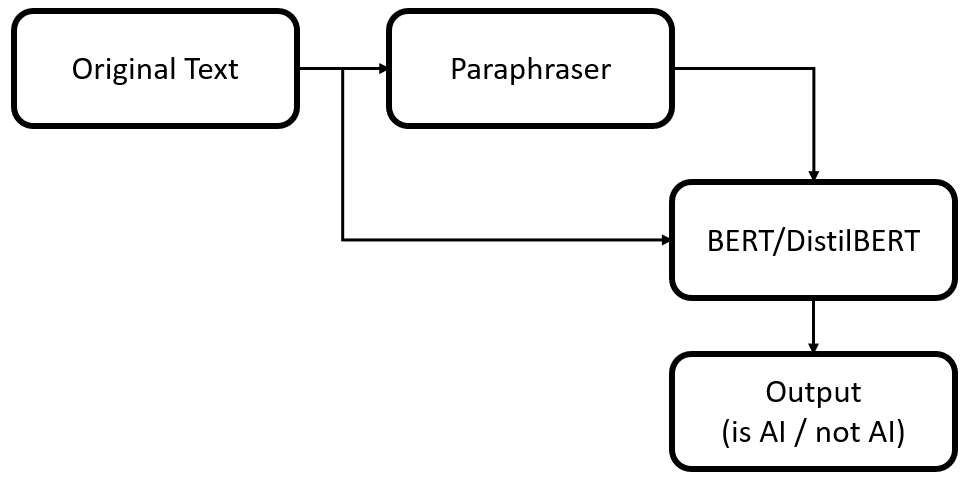
\includegraphics[width=0.5\textwidth]{structure.png}
\caption{Overall structure of the model.}
\label{fig:structure}
\end{figure}
\null\quad In the preliminary stages of model development, we encountered two predominant challenges that necessitated resolution.
The first challenge pertained to the acquisition of a sufficiently large dataset encompassing both human-authored journalism and machine-created journalistic content.
This issue was further exacerbated when our focus was narrowed to Korean corpora specifically, due to its limited availability. \\
\null\quad The second challenge was the notable disproportion in the amount of publicly accessible human-authored journalism compared to its machine-generated counterpart.
This discrepancy in data distribution could potentially culminate in a class imbalance problem,
thereby predisposing the model towards predicting news articles as being human-authored. \\
\null\quad To effectively navigate these challenges, we embarked on the creation of our own datasets.
This was accomplished by sourcing publicly available Korean news online and subsequently paraphrasing these articles with the assistance of one open source, and one closed sourcec Large Language Models with text-to-text generation capabilities.
This approach enabled us to compile a dataset with an equal representation of human-authored and machine-generated news.
It also held the potential to create a dataset of adequate size to facilitate the training of a robust model. \\
\null\quad Upon successful compilation of the dataset, we initiated the process of model development.
Given the constraints on computational resources, we made the strategic decision to leverage a pre-existing BERT model, rather than constructing a new one from scratch. \\
\null\quad Ultimately, an isolated segment of the dataset, earmarked specifically for testing purposes, was employed to gauge the performance of our fine-tuned model.
For the sake of comparison, these tests were also conducted on baseline models using a similarly sized testing dataset,
thereby allowing us to juxtapose the effectiveness of our model against existing frameworks.

\section{Experiments}
\null\quad The development of our model entailed the execution of numerous experiments, conducted across three distinct stages.
The initial stage, focused on dataset acquisition, involved testing several LLMs known for their text generation capabilities.
Our main objective at this stage was to identify which combination of models and hyperparameters would lead to the generation of text most closely resembling human-authored content.
Among the models subjected to testing were base LLaMA 2, beomi's Korean fine-tuned version of LLaMA 2, OpenChat 3.5, Google's T5, Google's Flan-T5, and GPT3.5.
Notably, due to limitations in our computational resources, we confined our experiments to the 7B and 13B models.
We further explored the influence of various hyperparameters on the output, including temperature, top\_p, and repetition\_penalty.
Our findings from these experiments indicated that the most optimal configuration for our specific needs comprised of the OpenChat 3.5 and GPT3.5 models, with a temperature setting of 0.7 and a top\_p value of 0.8. \\
\null\quad In the subsequent phase of our investigation, we assessed a multitude of foundational models renowned for their prowess in text classification, alongside an array of hyperparameters.
The objective was to discern the most efficacious amalgamation that would yield superior model performance.
Our empirical scrutiny was predominantly focused on two prominent models: BERT and DistilBERT (Sanh, V. et. al. 2019), a distilled variant of BERT optimized for speed and efficiency.
Our initial findings were intriguing; under the default parameter settings, DistilBERT demonstrated heightened performance.
However, as we extended the training duration and delved into hyperparameter optimization, BERT began to exhibit a marginal yet consistent edge over DistilBERT.
This phenomenon can be attributed to BERT's deeper and more complex architecture, which, despite requiring more computational resources and time,
has the capacity to capture nuanced patterns in the data that simpler models like DistilBERT might overlook. \\
\null\quad The concluding stage of our experimentation was characterized by the evaluation of diverse hyperparameters.
Alterations to weight decay, learning rate, and the epsilon parameter within the Adam optimization algorithm did not yield any substantial performance gains.
However, the introduction of a warmup step, constituting 10\% of the total training iterations, was instrumental in significantly elevating the performance benchmarks.
This enhancement can be ascribed to the warmup step's role in facilitating a more gradual and controlled increase in the learning rate,
which in turn aids the model in stabilizing its weights in the initial epochs, effectively preventing premature convergence to suboptimal minima. \\
\null\quad Concurrently, we observed an uptick in the loss metric beyond a certain threshold in the training epochs, indicative of the model's stagnation or potential overfitting.
To mitigate this, we instituted an early stopping protocol, which ceases training upon the cessation of improvement in the model's validation set performance.
This strategy was fundamental in preserving the model's generalizability and forestalls the overlearning of training set peculiarities.
Collectively, the calibration of the warmup steps and the implementation of early stopping have been pivotal in the refinement of our model, culminating in a more robust and generalized predictive performance.

\section{Dataset}
\null\quad As elucidated in the preceding sections, the dataset under consideration is constituted by an aggregation of news articles that are readily accessible to the public and originate from a variety of Korean news media outlets.
In tandem with these human-authored articles, the dataset also encompasses articles that have been machine generated.
It is imperative to note that these machine-generated articles are not original creations of the machine, but rather, they are paraphrased versions of the human-authored articles. \\
\null\quad This paraphrasing task was executed by a select group of LLMs that demonstrate proficiency in text-to-text generation.
The majority of the paraphrased articles were processed using the OpenChat 3.5 model, which was operated locally.
This choice of execution was predominantly guided by the financial constraints that were in play, which led to limited funds being available for conducting API calls to the OpenAI GPT-3.5 API with high frequency.

\section{Computing Resources}
Our experiments were conducted utilizing the following computing resources:

\begin{table}[ht]
\centering
\begin{tabular}{l c c}
\hline
Component & Computer 1 & Computer 2 \\
\hline
CPU & AMD Ryzen 5800X & Intel i7 4790 \\
GPU & Nvidia RTX 3060Ti & Nvidia GT730 \\
RAM & 24GB & 24GB \\
\hline
\end{tabular}
\caption{Specifications of Computing Resources}
\label{tab:computing_resources}
\end{table}

Computer 1 was utilized for all stages of development, while Computer 2 was occasionally used to perform API calls to OpenAI GPT3.5 during the dataset collection stage.

\section{Comparison with Baseline}
\begin{table}[ht]
\centering
\begin{tabular}{l c c c}
\hline
Metric & Our Model & Smodin & ZeroGPT \\
\hline
Accuracy & 0.7622 & 0.4211 & 0.5172 \\
Precision & 0.7279 & 0.4286 & 0.9918 \\
Recall & 0.8217 & 0.6626 & 0.0611 \\
F1 Score & 0.7719 & 0.5217 & 0.1250 \\
AUROC & 0.8570 & 0.4267 & 0.5268 \\
\hline
\end{tabular}
\caption{Performance metrics comparison.}
\label{tab:performance_comparison}
\end{table}
\null\quad For our given dataset of Korean human written articles and AI generated articles, our model demonstrated a superior accuracy of 0.7622,
which indicates a substantial improvement over Smodin and ZeroGPT, which scored 0.4211 and 0.5172, respectively.\\
\null\quad Precision, a metric that assesses the proportion of true positives over the total predicted positives, was highest in ZeroGPT with 0.9918. 
However, this is misleading without considering recall, as ZeroGPT considerably underperformed in that aspect with a mere 0.0611, compared to our model's 0.8217. 
This suggests that while ZeroGPT was precise, it failed to identify the majority of AI-generated articles. \\
\null\quad Furthermore, our model's F1 Score, which is the harmonic mean of precision and recall, stood at 0.7719, outpacing both Smodin and ZeroGPT by substantial margins.
This score represents a balanced approach between precision and recall, making it a more reliable indicator of a model's performance. \\
\null\quad Lastly, the Area Under the Receiver Operating Characteristic curve (AUROC), an aggregate measure of performance across all classification thresholds, was highest for our model at 0.8570.
This further substantiates our model's robustness in distinguishing between human and machine-generated content written in Korean.

\section{Conclusion}
\null\quad In conclusion, the comprehensive experimentation and methodical optimization of our model have been instrumental in its ability to accurately differentiate between human-written and AI-generated Korean journalism content.
The initial stage of dataset acquisition and model testing revealed the ideal parameters that simulate human-like text generation, providing a robust foundation for our subsequent analysis.
Our examination of foundational text classification models underscored BERT's superior capability to discern complex patterns in the data, outperforming its distilled counterpart, DistilBERT, especially upon extensive hyperparameter tuning and prolonged training. \\
\null\quad Throughout our rigorous testing phases, we not only honed in on the most effective model configurations but also refined our training process with strategic interventions such as the introduction of warmup steps and early stopping protocols.
These adjustments have been paramount in enhancing model generalizability and precluding overfitting, thereby ensuring a more reliable and consistent performance. \\
\null\quad The empirical results underscore our model's proficiency with an accuracy of 0.7622, significantly surpassing that of existing models such as Smodin and ZeroGPT.
The balance of precision and recall, as evidenced by a commendable F1 score of 0.7719, along with the highest AUROC score of 0.8570 further validate the model's effectiveness. \\
\null\quad Nevertheless, it is prudent to acknowledge that our model's comparative success may be, in part, attributed to the nature of the dataset it was trained on.
The dataset, being tailored for this experiment, may have inadvertently favored our model's learning mechanisms, skewing the results in its favor.
It is conceivable that Smodin and ZeroGPT, might perform differently under varying conditions and datasets. \\
\null\quad Consequently, to ascertain the generalizability and robustness of our findings, further investigative efforts are warranted. 
Future research endeavors should consider expanding the scope of the datasets, incorporating a broader and more diverse collection of samples that could challenge and potentially refine the model's predictive capabilities.
Moreover, it would be beneficial to explore the use of additional paraphrasing models to further generate paraphrased articles, which could provide a more rigorous testbed for our model's detection efficacy.
In the same vein, experimenting with other foundational classifier models may yield insightful comparative analyses, contributing to a more nuanced understanding of the strengths and weaknesses of our approach.
This comprehensive future work could ultimately lead to the development of more sophisticated models that excel in a variety of contexts and maintain high performance even when confronted with novel and complex data. \\

\bibliographystyle{unsrt}
\bibliography{references}
Jiang, G. (2023, May 30). Is AI-generated content actually detectable?: College of Computer, Mathematical, and Natural Sciences: University of Maryland. College of Computer, Mathematical, and Natural Sciences | University of Maryland. https://cmns.umd.edu/news-events/news/ai-generated-content-actually-detectable 

Hu, X., Chen, P. Y., \& Ho, T. Y. (2023). RADAR: Robust AI-Text Detection via Adversarial Learning. arXiv preprint arXiv:2307.03838.

Mitchell, E., Lee, Y., Khazatsky, A., Manning, C. D., \& Finn, C. (2023). Detectgpt: Zero-shot machine-generated text detection using probability curvature. arXiv preprint arXiv:2301.11305.

Devlin, J., Chang, M.-W., Lee, K., \& Toutanova, K. (2018). BERT: Pre-training of deep bidirectional Transformers for language understanding. arXiv preprint arXiv:1810.04805

Sanh, V., Debut, L., Chaumond, J., \& Wolf, T. (2019). DistilBERT, a distilled version of BERT: smaller, faster, cheaper and lighter. arXiv preprint arXiv:1910.01108

Trusted GPT-4, CHATGPT and AI detector tool by zerogpt. AI Detector - Accurate Chat GPT, GPT4 \& AI Text Checker Tool. (2023). \url{https://www.zerogpt.com/}

Free ai content detector. Smodin. (203). \url{https://smodin.io/ai-content-detector}
\end{document}